%%%%%%%%%%%%%%%%%%%%%%%%%%%%%%%%%%%%%%%%%%%%%%%%%%%
%% LaTeX book template                           %%
%% Author:  Amber Jain (http://amberj.devio.us/) %%
%% License: ISC license                          %%
%%%%%%%%%%%%%%%%%%%%%%%%%%%%%%%%%%%%%%%%%%%%%%%%%%%

%\documentclass[a4paper,11pt]{book}
\documentclass[b5paper,8pt]{book}
\usepackage{geometry}
\usepackage[T1]{fontenc}
\usepackage[utf8]{inputenc}
\usepackage{lmodern}
%%%%%%%%%%%%%%%%%%%%%%%%%%%%%%%%%%%%%%%%%%%%%%%%%%%%%%%%%
% Source: http://en.wikibooks.org/wiki/LaTeX/Hyperlinks %
%%%%%%%%%%%%%%%%%%%%%%%%%%%%%%%%%%%%%%%%%%%%%%%%%%%%%%%%%
\usepackage{hyperref}
\usepackage{graphicx}
\usepackage[english]{babel}

\usepackage{listings}
\usepackage{color}

\usepackage{algorithm}
\usepackage{algorithmic}

\usepackage{subfig}
\usepackage{amsmath}
\usepackage[makeroom]{cancel}

\usepackage{tcolorbox}

\usepackage{caption}

\usepackage[utf8]{inputenc}
\usepackage{imakeidx}
\usepackage{hyperref}

%\usepackage[spanish]{babel}
%\usepackage[usenames, dvipsnames]{color}
\definecolor{dkgreen}{rgb}{0,0.6,0}
\definecolor{gray}{rgb}{0.8,0.8,0.8}
\definecolor{mauve}{rgb}{0.58,0,0.82}
\definecolor{comments}{rgb}{1,1,0}

\lstset{frame=tb,
  language=C++,
  backgroundcolor=\color{white},
  aboveskip=3mm,
  belowskip=3mm,
  showstringspaces=false,
  columns=flexible,
  basicstyle={\scriptsize\ttfamily},
  numbers=none,
  numberstyle=\tiny\color{gray},
  keywordstyle=\color{blue},
  commentstyle=\color{dkgreen},
  stringstyle=\color{mauve},
  breaklines=true,
  breakatwhitespace=true
  tabsize=3
}

%%%%%%%%%%%%%%%%%%%%%%%%%%%%%%%%%%%%%%%%%%%%%%%%%%%%%%%%%%%%%%%%%%%%%%%%%%%%%%%%
% 'dedication' environment: To add a dedication paragraph at the start of book %
% Source: http://www.tug.org/pipermail/texhax/2010-June/015184.html            %
%%%%%%%%%%%%%%%%%%%%%%%%%%%%%%%%%%%%%%%%%%%%%%%%%%%%%%%%%%%%%%%%%%%%%%%%%%%%%%%%
\newenvironment{dedication}
{
   \cleardoublepage
   \thispagestyle{empty}
   \vspace*{\stretch{1}}
   \hfill\begin{minipage}[t]{0.66\textwidth}
   \raggedright
}
{
   \end{minipage}
   \vspace*{\stretch{3}}
   \clearpage
}

%%%%%%%%%%%%%%%%%%%%%%%%%%%%%%%%%%%%%%%%%%%%%%%%
% Chapter quote at the start of chapter        %
% Source: http://tex.stackexchange.com/a/53380 %
%%%%%%%%%%%%%%%%%%%%%%%%%%%%%%%%%%%%%%%%%%%%%%%%
\makeatletter
\renewcommand{\@chapapp}{}% Not necessary...
\newenvironment{chapquote}[2][2em]
  {\setlength{\@tempdima}{#1}%
   \def\chapquote@author{#2}%
   \parshape 1 \@tempdima \dimexpr\textwidth-2\@tempdima\relax%
   \itshape}
  {\par\normalfont\hfill--\ \chapquote@author\hspace*{\@tempdima}\par\bigskip}
\makeatother

%%%%%%%%%%%%%%%%%%%%%%%%%%%%%%%%%%%%%%%%%%%%%%%%%%%
% First page of book which contains 'stuff' like: %
%  - Book title, subtitle                         %
%  - Book author name                             %
%%%%%%%%%%%%%%%%%%%%%%%%%%%%%%%%%%%%%%%%%%%%%%%%%%%

% Book's title and subtitle
\title{\Huge \textbf{ Project Euler}  \\ \huge Solutions}
% Author
\author{\textsc{David Esparza Alba}}

\date{}

\makeindex

\begin{document}

\frontmatter
\maketitle

\tableofcontents

\mainmatter%%%%%%%%%%%%%%%%%%%%%%%%%%%%%%%%%%%%%%%%%%%%%%%%%%%%%%%
\addcontentsline{toc}{chapter}{80 - Square root digital expansion}
\chapter*{80 - Square root digital expansion}

\index{square root} 
It is well known that if the square root of a natural number is not an integer, then it is irrational. The decimal expansion of such square roots is infinite without any repeating pattern at all.\\

The square root of two is 1.41421356237309504880..., and the digital sum of the first one hundred decimal digits is 475.\\

For the first one hundred natural numbers, find the total of the digital sums of the first one hundred decimal digits for all the irrational square roots.\\

\section*{Solution}

To solve this problem we used the method of \textit{Square Root by Subtraction} described by Jarvis \cite{square_root}. This method allows us to find the square root of an integer $n$.\\

The algorithm \ref{alg:square_root} receives an integer $n$ and returns the first one hundred decimal digits of $\sqrt{n}$. The value of $p$ is set according of the number of decimal digits we want to calculate. 

\begin{algorithm}[H]
\caption{$squareRoot(n)$}
\begin{algorithmic}
    \STATE $a = 5n$
    \STATE $b=5$
    \STATE $p=10^{101}$
    \WHILE{$b < p$}
        \IF{$a \geq b$}
            \STATE $a \gets a-b$
            \STATE $b \gets b + 10$
        \ELSE
            \STATE $a \gets a \times 100$
            \STATE $b \gets \lfloor b/10 \rfloor \times 100 + 5$
        \ENDIF
    \ENDWHILE
    \STATE $b \gets \lfloor b/100 \rfloor$
    \RETURN b
\end{algorithmic}
\label{alg:square_root}
\end{algorithm}
 
\addcontentsline{toc}{chapter}{91 - Right triangles with integer coordinates}
\chapter*{91 - Right triangles with integer coordinates}

\index{binary search}
The points $P(x_1, y_1)$ and $Q(x_2, y_2)$ are plotted at integer co-ordinates and are joined to the origin, $O(0,0)$, to form $\Delta OPQ$.

\begin{figure}[H]
    \centering
    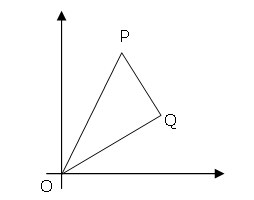
\includegraphics[scale=0.5]{images/pe911.png}
    \caption{}
    \label{fig:pe91a}
\end{figure}

There are exactly fourteen triangles containing a right angle that can be formed when each co-ordinate lies between 0 and 2 inclusive; that is, $0 \leq x1, y1, x2, y2\leq 2$.

\begin{figure}[H]
    \centering
    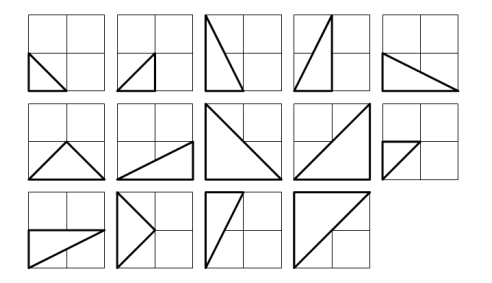
\includegraphics[scale=0.5]{images/pe912.png}
    \caption{}
    \label{fig:pe91b}
\end{figure}

Given that $0 \leq x1, y1, x2, y2 \leq 50$, how many right triangles can be formed?

\section*{Solution}

Since the coordinates are integer numbers in the range of $[0,50]$, a brute force approach will run in $O(n^4)$, with $n=50$ we are talking around six millions of operations, which looks reasonable to run in less than a minute. Now, in order to improve a little bit the running time we will do the following:

\begin{enumerate}
    \item Place the first point $(x_1,y_1)$ in the grid. This will take $O(n^2)$ to go trough the whole grid.
    \item For the other point $(x_2,y_2)$ iterate trough all values in the $y-axis$ and using a binary search obtain the $x-coordinate$, this part will run in $O(n \log n)$. Avoid to count the points where $y_2 = y_1$ and those where $x_2 = x_1$. To identify if we have found a valid coordinate we must check that the following statement is true (cosine law).
    
    $$
    x_1^2 + y_1^2 + (x_2-x_1)^2 + (y_2-y1)^2 - x_2^2 - y_2^2 = 0
    $$
    
    \item After counting the triangles f in step 2, we just need add $3n^2$, which is the number of right triangles with sides parallel to the $x$ and $y$ axis. 
    
\end{enumerate}

The running time of this solution is $O(n^3 \log n)$, which is around $7 \times 10^5$ operations. 
\addcontentsline{toc}{chapter}{95 - Amicable chains}
\chapter*{95 - Amicable chains}

\index{prime numbers}
The proper divisors of a number are all the divisors excluding the number itself. For example, the proper divisors of 28 are 1, 2, 4, 7, and 14. As the sum of these divisors is equal to 28, we call it a perfect number.\\

Interestingly the sum of the proper divisors of 220 is 284 and the sum of the proper divisors of 284 is 220, forming a chain of two numbers. For this reason, 220 and 284 are called an amicable pair.\\

Perhaps less well known are longer chains. For example, starting with 12496, we form a chain of five numbers:

$$
12496 \rightarrow 14288 \rightarrow 15472 \rightarrow  14536 \rightarrow  14264  (\rightarrow  12496 \rightarrow  ...)
$$

Since this chain returns to its starting point, it is called an amicable chain.\\

Find the smallest member of the longest amicable chain with no element exceeding one million.

\section*{Solution}

For a number $n$ the sum of the divisors less or equal than $n$ is given by

$$
S(n) = \prod_{i=1}^m \frac{p_i^{k_i+1} - 1}{p_i - 1}
$$

where 

$$
n = \prod_{i=1}^m p_i^{k_i}
$$

To generate the primes up to $10^6$ quickly we can use the \textit{Sieve of Eratosthenes}.\\

The idea is to mark the elements in a sequence and if we found a number that is already marked we will be able to obtain the length of the sequence and the starting/ending point of the cycle. We used an array $L$ and a counter to obtain the length of a cycle. For the example mentioned in the description we will have

\begin{align*}
    L_{12496} = 1 \\
    L_{14288} = 2 \\
    L_{15472} = 3 \\
    L_{14536} = 4 \\
    L_{14264} = 5
\end{align*}

The next value is $12496$ which is already marked, and the value of the counter is $6$, so the length of the sequence is $6 - L_{12496} = 5$. Also we can store in another array $X$ the starting/ending point of the cycle in each element of the chain, this is easily done using a recursive function.

\begin{align*}
    X_{12496} = 12496 \\
    X_{14288} = 12496 \\
    X_{15472} = 12496 \\
    X_{14536} = 12496 \\
    X_{14264} = 12496
\end{align*}

Sometimes we can start in a number that will led us to an already found cycle, just avoid counting the numbers found before entering the cycle.\\

Finally we just need to look for the number $k$ which $k = X_k$, and have the greatest $L_k$. Start moving trough that cycle to find the smallest element.
\addcontentsline{toc}{chapter}{100 - Arranged probability}
\chapter*{100 - Arranged probability}

\index{Diophantine quadratic}
If a box contains twenty-one coloured discs, composed of fifteen blue discs and six red discs, and two discs were taken at random, it can be seen that the probability of taking two blue discs, $P(BB) = (15/21)(14/20) = 1/2$.\\

The next such arrangement, for which there is exactly 50\% chance of taking two blue discs at random, is a box containing eighty-five blue discs and thirty-five red discs.\\

By finding the first arrangement to contain over $10^{12} = 1000000000000$ discs in total, determine the number of blue discs that the box would contain.

\section*{Solution}

Be $x$ the number of blue discs, and $y$ the total number of discs. We are looking values of $x$ and $y$ such as

\begin{align*}
    \left ( \frac{x}{y} \right ) \left ( \frac{x-1}{y-1} \right ) = \frac{1}{2} \\
    2x^2 - 2x = y^2 - y \\
    2x^2 - 2x - y^2 + y = 0
\end{align*}

A Diophantine equation is a polynomial equation with integer solutions only. A linear Diophantine equation is

$$
ax + by = c.
$$

Which can be solved using the \textit{Extended Euclidean} algorithm. For our case we have a quadratic Diophantine equation, and according to Mario Alpern's explanation \cite{quadratic_diophantine}, an equation of the form

$$
 ax^2 + bxy + cy^2 + dx + ey + f = 0
$$

has the following solutions:

\begin{align*}
    x_{n+1} &= Px_n + Qy_n + K \\
    y_{n+1} &= Rx_n + Sy_n + L
\end{align*}

For our specific equation the values of $P,Q,K,R,S,L$ are:

\begin{align*}
    P &= 3 \\
    Q &= 2 \\
    K &= -2 \\
    R &= 4 \\
    S &= 3 \\
    L &= -3
\end{align*}

The explanation of why these values is detailed in Mario Alpern's site.\\

Coming back to our problem. Using the formulas mentioned above, we only need to iterate though the different value of $x$ and $y$ until $y$ exceeds $10^{12}$.


\addcontentsline{toc}{chapter}{429 - Sum of squares of unitary divisors}
\chapter*{429 - Sum of squares of unitary divisors}

\index{prime numbers} \index{sum of combinations of products}
A unitary divisor $d$ of a number $n$ is a divisor of $n$ that has the property $gcd(d, n/d) = 1$.
The unitary divisors of $4! = 24$ are $1$, $3$, $8$ and $24$.
The sum of their squares is $1^2 + 3^2 + 8^2 + 24^2 = 650.$ \\

Let $S(n)$ represent the sum of the squares of the unitary divisors of $n$. Thus $S(4!)=650$. \\

Find $S(100000000!)$ modulo $1000000009$.

\section*{Solution}

First of all we must avoid calculating $n!$ directly. A better approach is to represent $n!$ as the product of its prime factors. For example, for $4!$ we have

$$
4! = 2^3 \times 3^1.
$$

Since we only care about those divisors with $gcd(d,n/d) = 1$, we must represent the number as the product of factors with exponent $1$. For $4!$ we obtain

$$
4! = 8^1 \times 3^1.
$$

The result we are looking for is the sum of the products of all combinations of the square of those factors. For this specific case we have that

$$
S(4!) = 1 + 8^2 + 3^2 + 8^2 3^2 = 650
$$

To calculate that sum we can use the following trick. Suppose there $3$ factors, $f_1, f_2, f_3$. The sum of the products of all combinations of those factors is given by:

$$
(1 + f_1)(1 + f_2)(1 + f_3) = 1 + f_1 + f_2 + f_3 + f_1f_2 + f_1f_3 + f_2f_3 + f_1f_2f_3.
$$

For our problem, if we have $m$ factors the solution would be given by

\begin{align*}
    S(n!) &= \prod_{i=1}^m (1 + f_i^2)\\
    &= \prod_{i=1}^m (1 + p_i^{2k_i}) 
\end{align*}


To obtain the value of $p_i^{2k^i}$ we can use binary exponentiation, in that case we will be dealing only with sums and products, and we can make use of the properties of modular arithmetic to keep the result modulo  $1000000009$.
\addcontentsline{toc}{chapter}{491 - Double pandigital number divisible by 11}
\chapter*{491 - Double pandigital number divisible by 11}

We call a positive integer double pandigital if it uses all the digits 0 to 9 exactly twice (with no leading zero). For example, 40561817703823564929 is one such number.\\

How many double pandigital numbers are divisible by 11?

\section*{Solution}

We can use some tricks to solve this problem. First of all, to know if a number is divisible by 11 we can sum all its digits in even positions and subtract the result by the sum of all digits in odd positions, if the result is divisible by 11, then the original number is also divisible by 11.\\

Knowing that we can generate only the digits in even positions using backtracking and keeping track of how many digits we have left. For that we can use an array $X$ of 10 elements, with initially $X_i = 2$, for each $i=0, \ldots, 9$, and every time we use the digit $k$ we decrease the value of $X_k$ by one.\\

When we have placed the ten digits in even positions we only need to calculate if the number is divisible by 11 and obtain the number of combinations to place the remaining digits in odd positions, this will be given by

$$
    \binom {10}{X_1,X_2,\ldots,X_9} = \frac{n!}{X_1!X_2!\cdots X_9!}
$$

The result is then added to our answer. \\

So far we will obtain a correct answer, but it can take a while to run.To improve the running time we can use memoization to store the results we are calculating in order to avoid to compute them again. To accomplish that we can represent the array $X$ as a base-3 number, and use a matrix $C$, so every time we are placing a digit in position $k$, we can store the result in $C_{kl}$, where $l$ is the base-10 representation of $X$.
\addcontentsline{toc}{chapter}{516 - 5-smooth totients}
\chapter*{516 - 5-smooth totients}

5-smooth numbers are numbers whose largest prime factor doesn't exceed 5.
5-smooth numbers are also called Hamming numbers.
Let $S(L)$ be the sum of the numbers n not exceeding $L$ such that Euler's totient function $\phi(n)$ is a Hamming number.\\

$S(100)=3728.$\\

Find $S(10^{12})$. Give your answer modulo $2^{32}$.

\section*{Solution}

To solve this problem we do the following:

\begin{itemize}
    \item Store all numbers of the form $2^a 3^b 5^c$ in an array $H$.
    \item Obtain all prime numbers of the form $2^a 3^b 5^c + 1$ greater than 5 and store them in an array $T$. Since a prime number $p$ has $\phi(p) = p-1$, then all elements in $T$ comply with $\phi(2^a 3^b 5^c + 1) = 2^a 3^b 5^c$.
    \item Sort the elements in $H$ and $T$.
    \item Add the sum of all elements in $H$ to the answer.
    \item Multiply each element in $H$ to all combinations of products of the elements in $T$ and add those values to the answer. Since the $\phi$ function is multiplicative , then for a any prime $p$ in $T$ we have 
    
    \begin{align*}
        \phi(p 2^a 3^b 5^c) &= \phi(p) \phi(2^a) \phi(3^b) \phi(5^c) \\
        &= (2^x 3^y 5^z) (2^{a-1}) (3^{b-1}) (5^{c-1}) \\
        &= 2^{x+a-1} 3^{y+b-1} 5^{z+c-1}
    \end{align*}
    
    To this last part we can use backtracking, just be careful to not multiply the same prime more than once, since $\phi(nm) = \phi(n)\phi(m)$ only if $gcd(n,m) = 1$.
    
\end{itemize}


%\include{chapter}
%\appendix
%\include{appendix}

\backmatter%%%%%%%%%%%%%%%%%%%%%%%%%%%%%%%%%%%%%%%%%%%%%%%%%%%%%%%
%%%%%%%%%%%%%%%%%%%%%%%% referenc.tex %%%%%%%%%%%%%%%%%%%%%%%%%%%%%%
% sample references
% "computer science"
%
% Use this file as a template for your own input.
%
%%%%%%%%%%%%%%%%%%%%%%%% Springer-Verlag %%%%%%%%%%%%%%%%%%%%%%%%%%

%
% BibTeX users please use
% \bibliographystyle{}
% \bibliography{}
%
% Non-BibTeX users please use
\begin{thebibliography}{99.}

\bibitem{square_root} Frazer Jarvis (2002)
\href{http://www.afjarvis.staff.shef.ac.uk/maths/jarvisspec02.pdf}{http://www.afjarvis.staff.shef.ac.uk/maths/jarvisspec02.pdf}

\bibitem{quadratic_diophantine} Mario Alpern
\href{https://www.alpertron.com.ar/CUAD.HTM}{https://www.alpertron.com.ar/CUAD.HTM}

\bibitem{hungarian} Dénes Kőnig and Jenő Egerváry (1955)
\href{https://en.wikipedia.org/wiki/Hungarian\_algorithm}{https://en.wikipedia.org/wiki/Hungarian\_algorithm}

\bibitem{wilson_theorem} Ibn al-Haytham
\href{https://en.wikipedia.org/wiki/Wilson\%27s\_theorem}{https://en.wikipedia.org/wiki/Wilson\%27s\_theorem}


\end{thebibliography}

\printindex

%%%%%%%%%%%%%%%%%%%%%%%%%%%%%%%%%%%%%%%%%%%%%%%%%%%%%%%%%%%%%%%%%%%%%%

\end{document}





